\documentclass[tikz,border=10pt]{standalone}
\usepackage{tikz}
\usetikzlibrary{scopes}
\usepackage{verbatim}
\usetikzlibrary{calc,angles,patterns,quotes, arrows}
\usetikzlibrary{positioning}




\begin{document}

\def\iangle{35} % Angle of the inclined plane
\def\down{-90}
\def\arcr{0.5cm} % Radius of the arc used to indicate angles
\def\ang{30}
\def\radius{5em} % radiaus of a timber
\def\dotsize{0.1em}
\def\nsize{0.5}


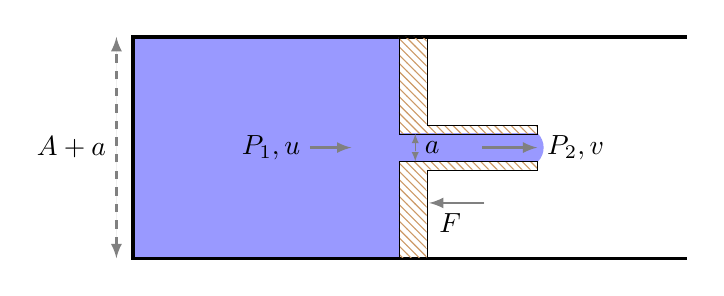
\begin{tikzpicture}[
    force/.style={>=latex, thick,draw=gray,fill=gray},
    axis/.style={densely dashed,gray},
    M/.style={rectangle,draw,fill=lightgray,minimum size=0.5cm,thin},
    m/.style={rectangle,draw=black,fill=lightgray,minimum size=0.3cm,thin},
    plane/.style={draw=black,fill=blue!10},
    string/.style={draw=red, thick},
    pulley/.style={thick},
    timber-fill/.style={pattern=north west lines, pattern color=brown!80}
]

\pgfdeclarelayer{water}
\pgfsetlayers{water, main}

\node (lower_exit) {};
\draw[very thick] (lower_exit.center)  -- ++(-20em, 0) node[midway] (lower_middle){} 
                                       -- ++(0, 8em) 
                                       -- ++(20em, 0) node[midway] (upper_middle){};

\path (lower_exit.center)  -- ++(-20em, 0) node (lower_corner){} 
                           -- ++(0, 8em)  node (upper_corner){}
                           -- ++(20em, 0);

\filldraw[timber-fill, line width=0.01em] (lower_middle.west) 
                                           -- ++(0, 3.5em) node (bottom_in_corner){}
                                           -- ++(5em, 0) node (bottom_out_corner){} 
                                           -- ++(0, -0.3em)
                                           -- ++(-4em, 0)
                                           -- ++(0, -3.2em) -- cycle;

\filldraw[timber-fill, line width=0.01em] (upper_middle.west) 
                                           -- ++(0, -3.5em) node (top_in_corner){}
                                           -- ++(5em, 0) node (top_out_corner){} 
                                           -- ++(0, 0.3em)
                                           -- ++(-4em, 0)
                                           -- ++(0, 3.2em) -- cycle;


\path (lower_corner) -- node[midway](under_label){} (lower_middle.west);
\path (upper_corner) -- node[midway](above_label){} (upper_middle.west);
\path (above_label) -- node[midway](left_label) {$P_1, u$} (under_label);
\draw[force, ->] (left_label.east) -- ++(1.5em, 0);

\path (top_out_corner) -- node[midway, right](right_label){$P_2, v$} (bottom_out_corner);
\draw[force, ->] ([xshift=-2em]right_label.west) -- (right_label.west);

\draw[force, dashed, <->] ([xshift=-0.25em]lower_corner.west) -- 
node[midway, left]{$A+a$} ([xshift=-0.25em]upper_corner.west);

\draw[force, dashed, <->, very thin] ([xshift=0.25em]top_in_corner.east) -- 
node[midway, right]{$a$} ([xshift=0.25em]bottom_in_corner.east);

\draw[force, ->] ([yshift=2em, xshift=2.3em]lower_middle.east) -- 
                 ++(-2em, 0) node[below right] {$F$}; 

\begin{pgfonlayer}{water}
    \filldraw[blue!40, fill=blue!40] (lower_middle.west) 
    -- (lower_corner.center) 
    -- (upper_corner.center)
    -- (upper_middle.west)
    -- (top_in_corner.center)
    -- (top_out_corner.center) to[out=-45, in=45] (bottom_out_corner.center) 
    -- (bottom_in_corner.center)
    -- (lower_middle.west) 
    -- cycle;    
\end{pgfonlayer}                                           



\end{tikzpicture}



\end{document}
